% \newpage

\begin{figure}[!h]
    \begin{subfigure}{\linewidth}
        \centering
        % \hspace{-0.8cm}
        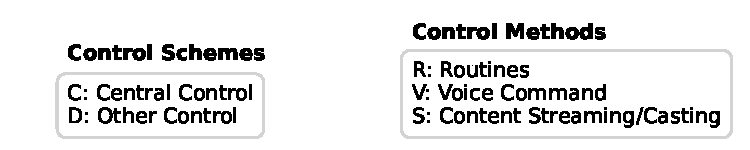
\includegraphics[width=0.5\textwidth]{ControlInContext/figures/control_schemes_legend_split.pdf}
        \vfill
        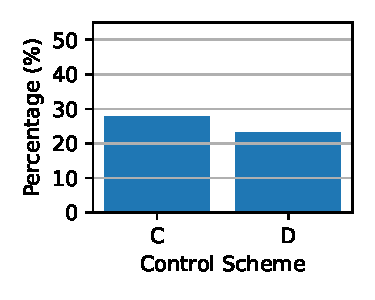
\includegraphics[width=0.225\textwidth]{ControlInContext/figures/control_schemes_popularity.pdf}
        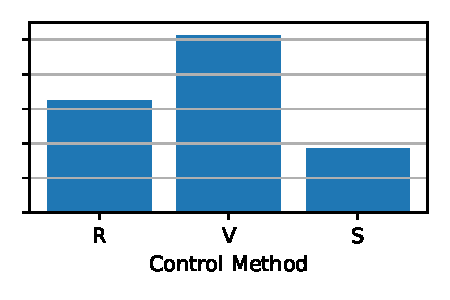
\includegraphics[width=0.27\textwidth]{ControlInContext/figures/control_methods_popularity.pdf}
        \caption{Percentage of participants using each control scheme/method.}
    %     \Description{
    % Bar charts showing participant usage of control schemes and control methods in percentages.

    % The left chart shows control scheme preferences: approximately 30\% of participants use Central Control (C), and about 25\% use Other Control (D).

    % The right chart shows control method preferences: Voice Command (V) is the most used at just over 50\%, followed by Routines (R) at around 30\%, and Content Streaming/Casting (S) at under 20\%.

    % Legends clarify abbreviations for both schemes and methods.
    %     }
        \label{fig:control-scheme-popularity}
    \end{subfigure}
    \hfill
    \begin{subfigure}{\linewidth}
        \centering
        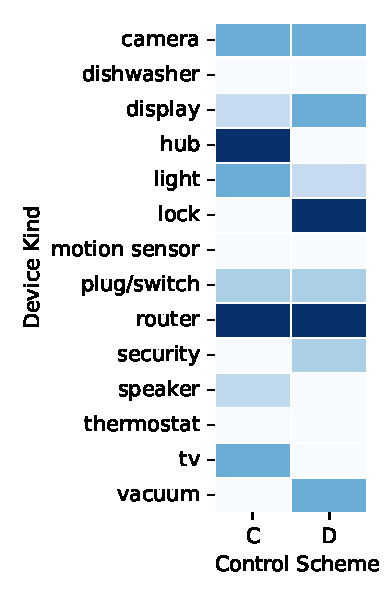
\includegraphics[width=0.25\linewidth]{ControlInContext/figures/control_schemes_vs_dev_kind_pc.pdf}
        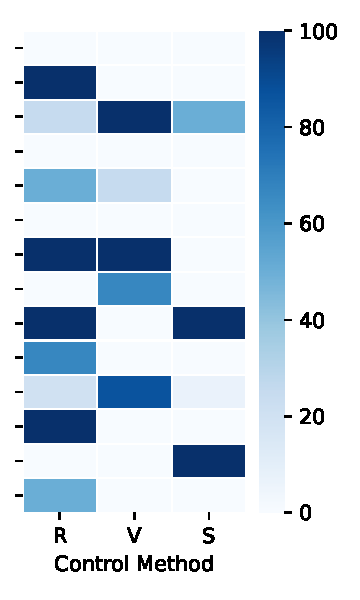
\includegraphics[width=0.235\linewidth]{ControlInContext/figures/control_methods_vs_dev_kind_pc.pdf}
        \caption{Percentage of participants using each control scheme/method vs. device kind. Each cell's color shows the percentage of participants falling into it who choose the respective control scheme or method.
        % \todo{Add some text to account for devices that have possibly more functionalities than described. put it here.}
        Participants may refer to a device with a different description from how they most commonly use it, leading to an occasional discrepancy between the device kind and the control method used to interact with it; for example, a participant may refer to Alexa as only a smart speaker, when it is also a Hub~\cite{wang2020want,singh2018users, georgiev2018smart}.
        }
        % \Description{
        % Heatmaps showing participant usage of control schemes and control methods across 14 device kinds.

        % The left heatmap compares Central Control (C) and Other Control (D) schemes. Device types with strong central control usage include routers, hubs, and displays, while locks and vacuums are more often associated with less centralized control. Some devices, like plugs/switches and cameras, show similar usage across both schemes.

        % The right heatmap compares three control methods: Routines (R), Voice Command (V), and Content Streaming/Casting (S). Routines are most associated with dishwashers, motion sensors, and thermostats. Voice Command is commonly used with displays, speakers, and motion sensors. Content Streaming is primarily used with routers and thermostats.

        Color intensity reflects the percentage of participants using a control scheme or method for each device kind, with darker cells indicating higher percentages.
}
        \label{fig:control-scheme-popularity-vs-dev-kind}
    \end{subfigure}
    \caption{Percentages of participants using each control scheme/method independently and in relation to the interacting devices. The percentages for the different options of control schemes and methods do not add up to 100\% since the participants could provide multiple answers. %\todo{PUT FIGURE 1a and 1c in the appendix, and make figure b stand on its own and wrap text around it so it doesn't look weird with the one column format}. (Q16, \Cref{appdx:survey:control}). %\todo{Figure out the column width balance}
    }
    \label{fig:control-schemes-appdx}
\end{figure}

\section{Further Results}
\label{appdx:further-results}


% \newpage


In this section, we present further results from our survey responses, particularly with regard to how the participant used a particular device they interacted with often.\footnote{Within the survey, we used terms like central and per-device control that the participants can easily understand before the interview stage. We later analyzed the survey data from our spectrum-based lens. See \Cref{appdx:survey:control} for the actual questions.}
Among control methods, voice commands were the most popular (\Cref{fig:control-scheme-popularity}), particularly among participants who owned less than 10 devices. The popularity is likely due to the simplicity and ease of issuing commands via voice for certain groups of devices, such as speakers and displays. Routines were the second most common control method. They were used more consistently by participants with a moderate number of devices, typically owning more than 15 devices (\Cref{fig:control-scheme-popularity-vs-dev-no}). Content streaming and casting also maintained a steady usage across participants, likely driven by the types of devices they owned, such as smart TVs or speakers, which are inherently designed for such interactions (\Cref{fig:control-scheme-popularity-vs-dev-kind}).

As \Cref{fig:control-scheme-popularity-vs-dev-kind} shows, control scheme preferences differ across device types. Non-central types of control remain popular among participants with devices that require more granular or custom interactions, such as security systems or vacuums, where direct control over specific features is necessary. We also observe that participants usually choose to control a device exclusively with either routines or voice commands but not both.

